\documentclass[a4paper,fontset=mac]{ctexart}
\usepackage[margin=1in]{geometry}
\usepackage{booktabs}
\usepackage{tabularx}
\usepackage{graphicx}
\usepackage{hyperref}
% \hypersetup{hidelinks}

\title{论文阅读报告}
\author{PB24000150 李欣宸}
\date{\today}

\begin{document}

\maketitle

此系《深度学习基础》课程论文阅读报告作业，我选择的是 CVPR 2025 论文 {\it Sonata: Self-Supervised Learning of Reliable Point Representations}\footnote{\url{https://arxiv.org/abs/2503.16429}}。该论文的主题是点云模态的自监督表征学习，对应报告要求属于“多模态模型”的“自监督学习”。

\section{选择理由}

这篇论文是我在前段时间在课题组中阅读的论文中，引用量和知名程度相对比较高的一篇论文。我选择这篇文章的主要理由如下：

\paragraph{创新性} 该论文比较早地尝试了，在点云数据下，是否可以像图像自监督学习中的 DINO、MAE 一样，训练出一个可以直接迁移到多种下游任务的通用表征；该文是点云自监督学习领域中重要的工作之一。

\paragraph{典型性} 在实验方法上，该论文大量借鉴了其他模态的研究成果；自蒸馏、线性探测、零样本可视化都是自监督学习中常用的方法；虽然该论文针对点云模态，但该论文的阅读对我理解自监督学习的实验方法和整体方法论有很大帮助。

\section{主要内容}

该论文主要做了三点：1）分析了点云自监督学习中，现有训练和评价方式存在的“几何捷径”问题；2）提出了 Sonata 方法，针对几何捷径设计了新的训练策略；3）在多个室内和室外数据集上进行了大规模实验，验证了方法的有效性。

这篇论文要解决的问题是提升点云模态自监督学习的质量。相比只看完整微调后的最终结果，作者更关心一个问题：预训练出的点云特征本身是否可靠。这个问题对应到实验上，就是冻结主干后的线性探测、解码器探测，以及不带标签的特征可视化。

\paragraph{几何捷径与评价方式}

几何捷径是该论文旨在解决的核心问题。点云模态中，由于数据的采集方式特性，仅从点云的分布就可以推断很多几何特征；现有自监督学习方法的损失往往在开始的时候下降很快，后面难以下降，而这个下降的原因没有被深入研究；使用 PCA 可视化现有模型，可以发现编码器学到的大多为低级几何特征（比如面的朝向，高度，法向），真正的语义特征往往在用有监督学习训练出的解码器中才有所体现。这个现象被该论文称为“几何捷径”（geometric shortcut），即，自监督学习往往退化为只学习几何特征的平凡解。

“几何捷径”现象来源于点云模态和对比学习中数据增广（data augmentation）的失配。点云模态中，数据增广往往是对点云的旋转、缩放、平移、遮盖等操作；而点云网络本身的算子（如邻域构建、采样和聚合）都依赖于坐标信息。因此，即使输入特征被遮盖，模型仍然可以通过坐标和局部空间结构猜出很多低级几何信息。这样预训练任务看似被完成了，但模型学到的并不是稳定的语义表征。

由于该现象的特点，过去的点云自监督学习方法大多使用的，在新任务上微调编码器检查性能的方式，难以刻画这种现象。因此该文章借用了图像自监督学习中常用的线性探测和零样本可视化的方式，来评价点云自监督学习的表征质量。这些评价方式会尽量减少下游训练的补救能力，从而更直接地暴露表征是否只停留在低级几何层面。

\begin{figure}[htbp]
    \centering
    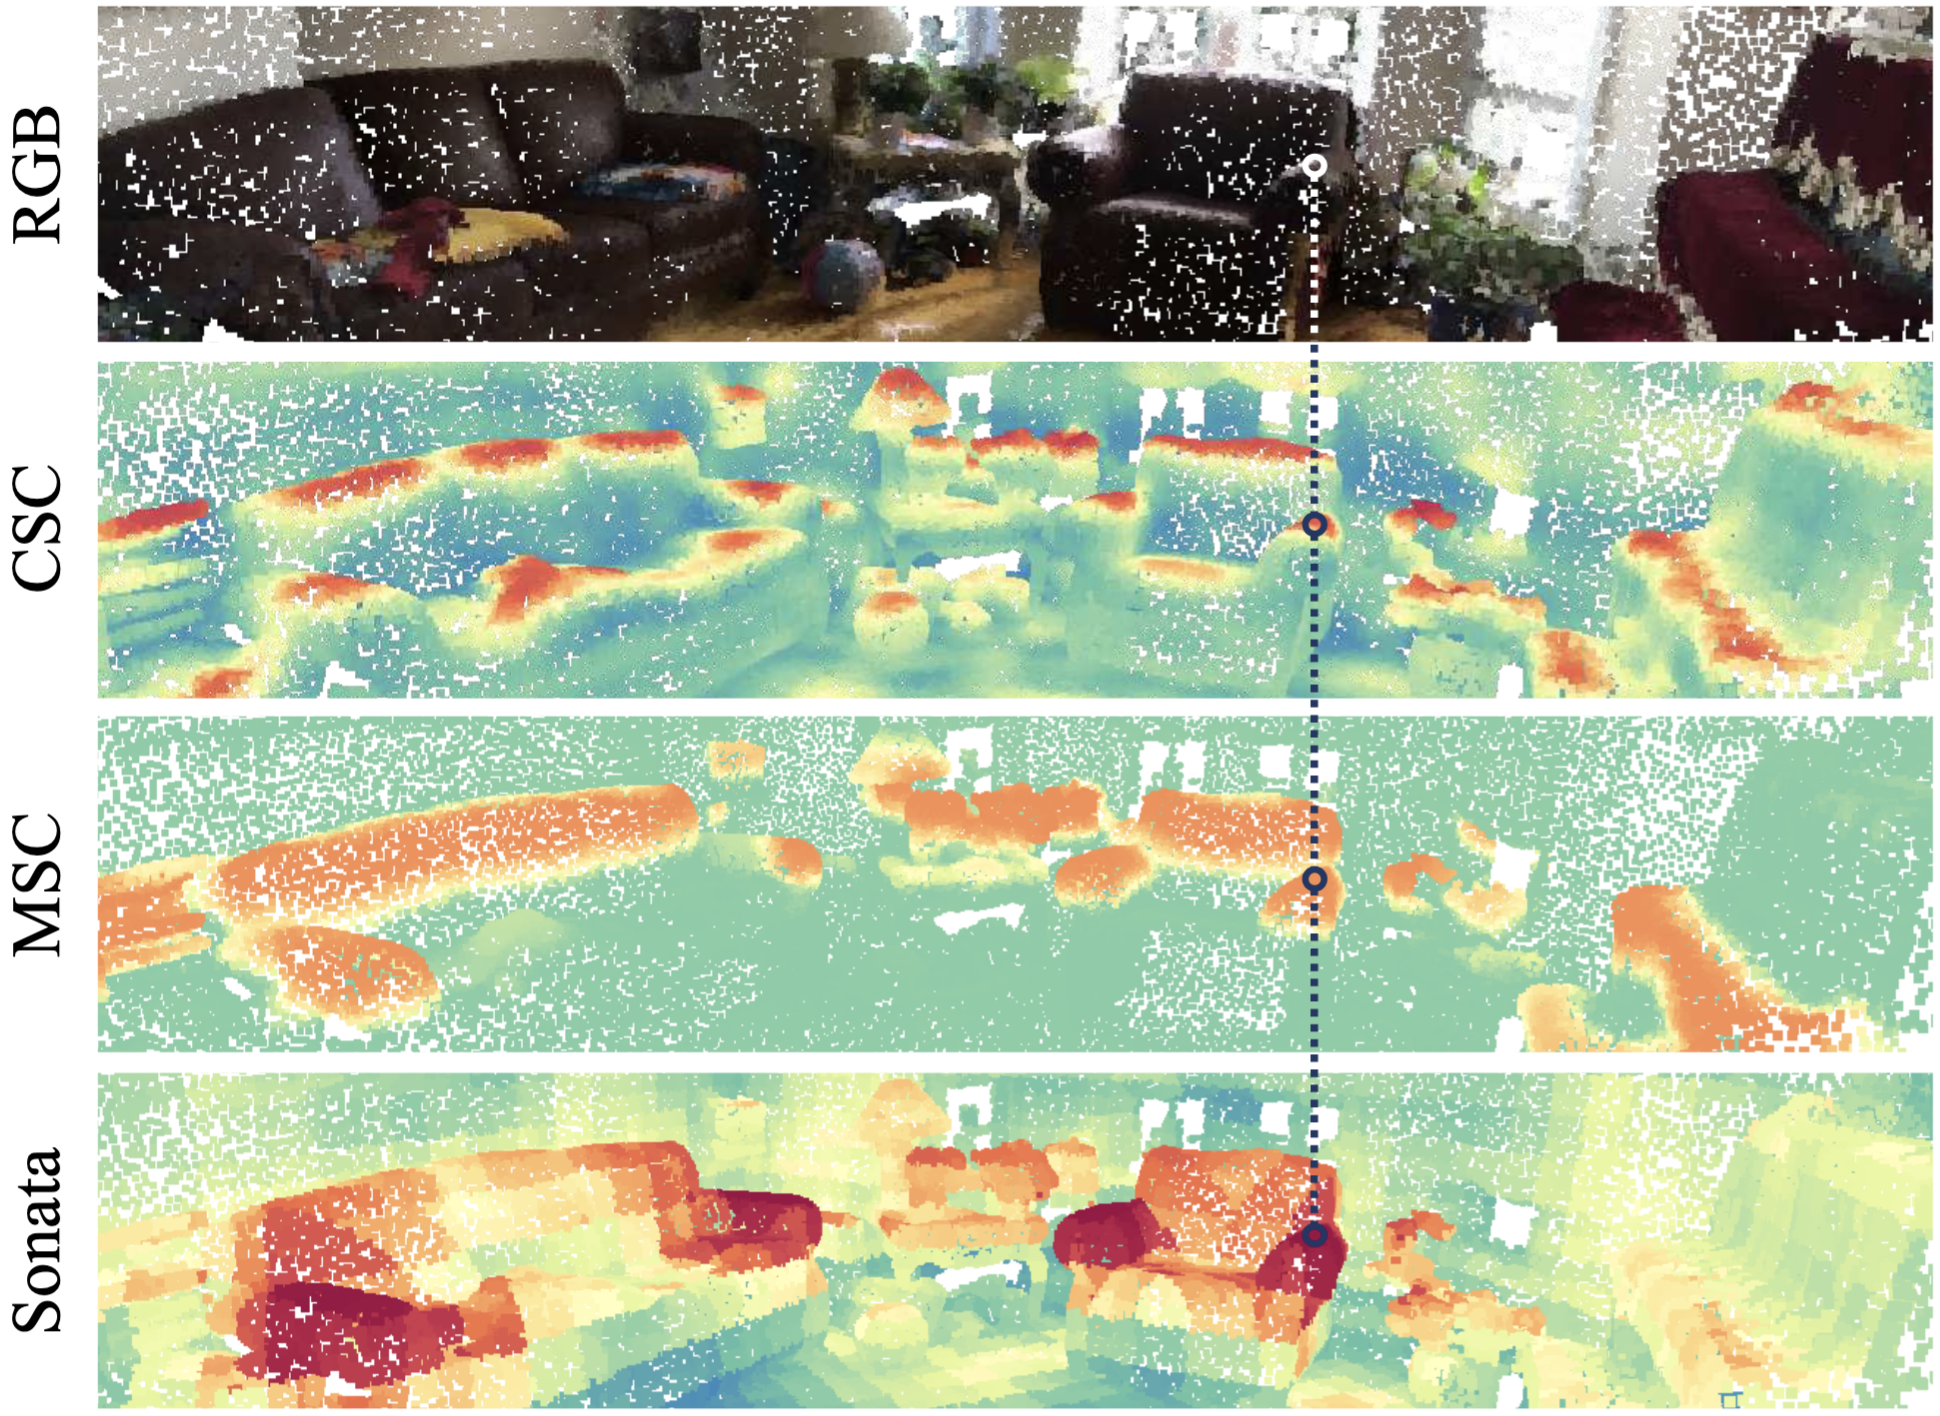
\includegraphics[width=0.78\textwidth]{figures/sonata_fig2.png}
    \caption{论文 Figure 2 中的几何捷径可视化。给定沙发扶手上的一个点，已有方法的相似度更多对应法向或高度，而 Sonata 更接近语义相似性。}
\end{figure}

\paragraph{Sonata 方法}

该论文的主要思路可以概括为两点：减弱坐标带来的捷径，增强模型对输入特征和上下文的依赖。

Sonata 的主体是点级自蒸馏。模型从同一个点云生成全局视图、局部视图和遮盖视图；学生网络处理更困难的局部/遮盖视图，教师网络处理信息更完整的全局视图，教师参数由学生参数的指数滑动平均得到。训练目标不是重建点云，而是让不同视图中对应或邻近的点具有一致的特征表示和聚类分配。

这一部分明显借鉴了 DINO/SwAV 一类图像自监督方法。SwAV 使用 Sinkhorn-Knopp 把样本到 prototype 的分配做成近似平衡分配，避免所有样本塌缩到少数簇；DINO/DINOv2 中也有中心化、锐化等防塌缩设计。Sonata 把这些技巧迁移到点云上：教师分支给出稳定目标，学生分支去匹配它，并用 Sinkhorn-Knopp 中心化、温度调度和 KoLeo 正则化维持特征空间的均衡。

围绕几何捷径，论文做了几项具体修改：

\begin{itemize}
    \item \textbf{移除解码器。} 自监督损失不再加在 U-Net 解码器的原始分辨率特征上，而是直接作用于 PTv3 编码器的较粗尺度特征，减少局部坐标细节泄漏。
    \item \textbf{特征上投影。} 只用最粗尺度特征会丢失多尺度上下文，因此作者把编码器特征无参数地逐级上投影，并与前一层特征拼接。
    \item \textbf{遮盖点坐标扰动。} 对被 mask 的点施加强高斯扰动，破坏局部空间关系，使模型不能只靠原始坐标完成任务。
    \item \textbf{渐进式任务调度。} mask 比例和 mask 尺寸从小到大逐渐增加，避免任务一开始过难，同时逐步压制几何捷径。
\end{itemize}

\begin{figure}[htbp]
    \centering
    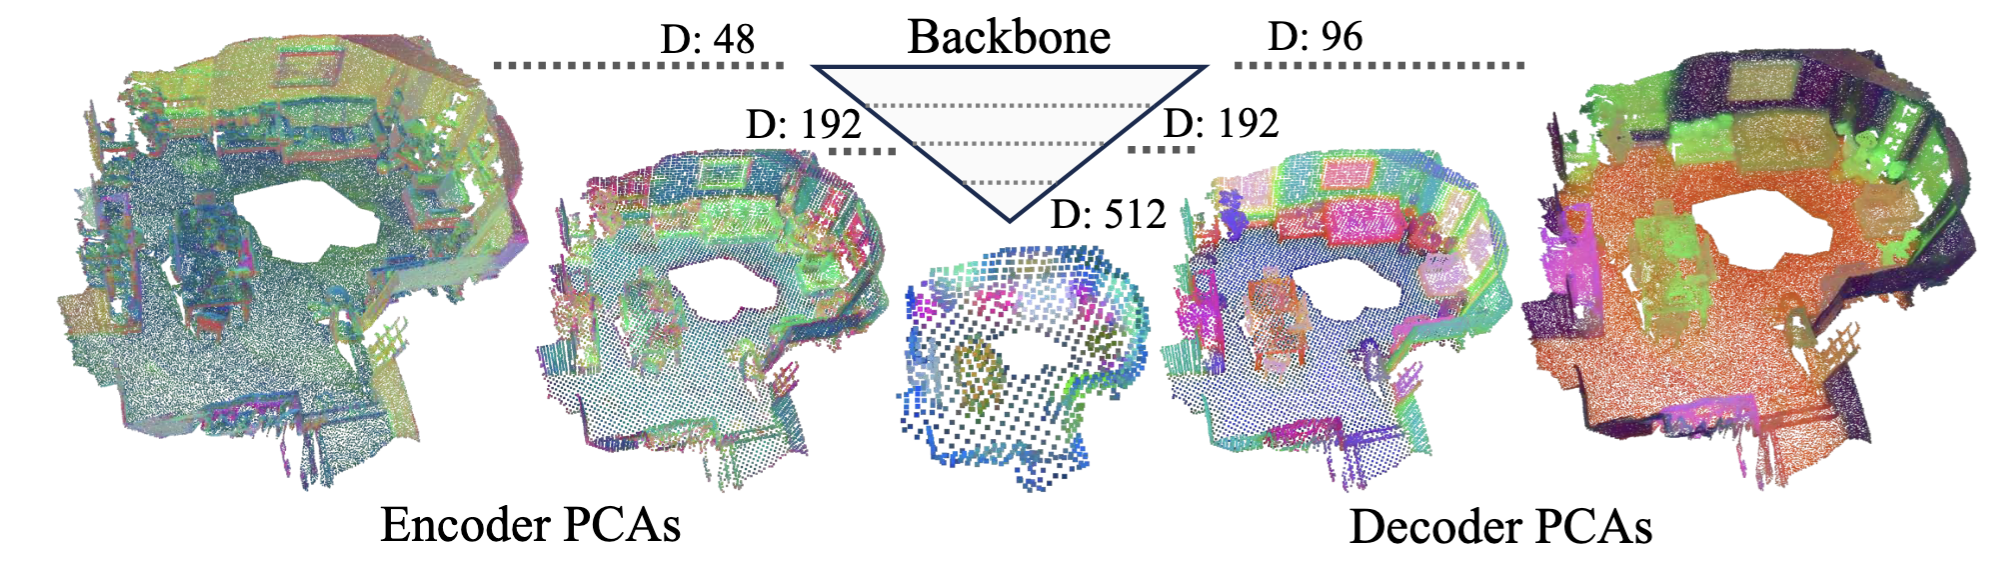
\includegraphics[width=0.78\textwidth]{figures/sonata_fig4.png}
    \caption{论文 Figure 4 展示了层级 backbone 中 encoder/decoder 特征的 PCA 可视化。encoder 中较粗尺度特征更分散，decoder 特征更偏向任务输出，这也是 Sonata 选择在 encoder 上做自监督的原因之一。}
\end{figure}

因此 Sonata 的创新不在于发明一个全新的网络结构，而在于把图像自监督的经验放到点云模态后，重新处理坐标信息、特征尺度和训练难度这三个问题。

\section{实验结果}

论文使用约 14 万个场景级点云进行预训练，数据来自 ScanNet、ScanNet++、S3DIS、ArkitScenes、HM3D、Structured3D 和 ASE 等数据集。主干网络使用 PTv3，评价方式包括线性探测、解码器探测和完整微调。

\begin{table}[h] \centering
  \begin{tabularx}{\textwidth}{>{\raggedright\arraybackslash}X >{\raggedleft\arraybackslash}p{0.18\textwidth} >{\raggedleft\arraybackslash}p{0.18\textwidth}}
    \toprule
    \textbf{方法} & \textbf{可学习参数比例} & \textbf{ScanNet mIoU} \\
    \midrule
    MSC 线性探测 & 0.2\% & 21.8 \\
    Sonata 线性探测 & 0.2\% & 72.5 \\
    Sonata 解码器探测 & 13\% & 79.1 \\
    Sonata 完整微调 & 100\% & 79.4 \\
    \bottomrule
  \end{tabularx}
  \caption{Sonata 在 ScanNet 语义分割上的参数效率结果}
\end{table}

最核心的结果是线性探测。Sonata 在 ScanNet 上把线性探测 mIoU 从 MSC 的 21.8\% 提升到 72.5\%，说明冻结后的点云表征已经有较强语义信息；解码器探测达到 79.1\%，和完整微调的 79.4\% 很接近，也说明编码器表征本身已经比较充分。

论文还比较了 Sonata 和投影到 3D 的 DINOv2 特征。DINOv2 的 ScanNet 线性探测 mIoU 为 63.1\%，Sonata 为 72.5\%，二者结合后可以进一步提升。这说明 Sonata 学到的不是图像语义的简单重复，而是包含了独立的 3D 信息。

在数据效率方面，只使用 1\% ScanNet 场景时，Sonata 完整微调达到 45.3\% mIoU，从头训练约为 25.8\%。考虑到点云标注成本很高，这一点也比较重要。完整微调时，Sonata 在 ScanNet、S3DIS、nuScenes、Waymo 和 SemanticKITTI 等数据集上也取得了较强结果。

\section{启发}

这篇文章是对自蒸馏技巧的典型应用，对点云自监督学习进行了深入的分析。阅读后我有以下几点启发：

\paragraph{自监督学习的梯度视角}

Sonata 中移除解码器这一点可以从梯度角度理解。如果自监督损失加在原始分辨率的 decoder 特征上，梯度会直接作用在很细的局部结构上，模型更容易强化高度、法向、局部平面这类低级几何特征；而把损失放在较粗尺度的 encoder 特征上，相当于限制了这条路径。遮盖点坐标扰动也是类似的作用：它不是单纯的数据增广，而且让梯度很难再沿着“复原局部坐标关系”这条路走。

\paragraph{评价方式的重要性}

作者使用可视化方法等多种手段，敏锐地观察到，虽然点云里的 mask 操作看起来和图像遮盖类似，但点云网络的邻域构建、采样和聚合都依赖坐标。也就是说，即使输入特征被遮住，模型仍然可能通过坐标恢复局部几何关系。这样 loss 会下降，但下降方向其实是“更会利用坐标”，而不是“更懂语义”。

对于衡量模型效果，如果只看完整微调，预训练表征的缺陷可能会被下游 decoder 或全量参数更新补掉。因此作者强调线性探测、decoder probing 和零样本可视化。我觉得这点对读论文也有帮助：一个方法是不是真的学到了通用表示，不能只看最终榜单分数，还要关注一些蕴藏在模型中间的可能更本质的指标。

\paragraph{点云表征和图像表征的互补性}

论文中 Sonata 和 DINOv2 特征结合后还能提升，这说明 3D 自监督不是简单复制图像语义。图像特征更强在纹理、颜色和外观语义，点云特征更强在空间结构和几何关系。后续如果做多模态 3D 表征，比较自然的方向不是只把图像特征投到点云上，而是设计一个互相蒸馏的训练过程。

\end{document}
